\documentclass[12pt]{article}
\usepackage{fullpage}
\usepackage{amsmath, amsfonts, amssymb, amsthm}
\usepackage{mathtools}
\usepackage{bm}
\usepackage{tikz}
\usepackage[section]{algorithm}
\usepackage{algpseudocode}
\usepackage{verbatim}
\usepackage{hyperref}
\usepackage{subcaption}
\usepackage{cleveref}
\usepackage[sort]{natbib}
\usepackage{complexity}
\usepackage{enumerate}
\usepackage[title]{appendix}
\usepackage{adjustbox}
\usepackage{xurl}

\newcommand{\ind}[1]{\mathbf{1}(#1)}

\newcommand{\prob}[1]{\mathbb{P}(#1)}
\newcommand{\varprob}[1]{\mathbb{P}\left(#1\right)}
\newcommand{\Var}[1]{\operatorname{Var}(#1)}

\newcommand{\maxAlpha}{\ensuremath{0.00025}}
\newcommand{\maxAlphaDiff}{\ensuremath{0.019}}


\newtheorem{theorem}{Theorem}
\numberwithin{theorem}{section}
\newtheorem{definition}[theorem]{Definition}
\newtheorem{lemma}[theorem]{Lemma}
\newtheorem{corollary}[theorem]{Corollary}
\newtheorem{conjecture}[theorem]{Conjecture}
\newtheorem{question}[theorem]{Question}

\title{Strongly Consistent Interval Estimates Based on Asymptotic Normality}
\author{Justin Rising\thanks{Philadelphia, PA\\email: \texttt{jkrising@gmail.com}}}


\begin{document}

\maketitle

\begin{abstract}
I exhibit a sequence of interval estimates $\hat{I}_n$ for an unknown population mean $\mu$ such that the length of $\hat{I}_n$ converges to zero in probability and $\prob{\mu \in \hat{I}_n}$ converges to one as n becomes large.  The analysis is based on an asymptotically tight upper bound for Gaussian quantiles that may be of independent interest.
\end{abstract}

\section{Introduction}
\label{sec_intro}

Every student who has taken an introductory class in statistics is familiar with the confidence intervals for the mean of an unknown population derived from the central limit theorem.  While these intervals have the correct asymptotic coverage probability, their coverage probability for a finite sample may be significantly lower~\citep{brown2001binomInt}.

However, the assumptions of the central limit theorem are quite weak, and it seems reasonable to believe that under stronger conditions we can place some bound on the excess error probability of these intervals.  This was confirmed in~\cite{hall1995coverage}, where regularity conditions were given that bound the coverage probability by $1 - \alpha - O(n^{-1})$.

In this paper, we will see that this bound is sufficient to construct a sequence of interval estimates with a property referred to in~\cite{rising2023orderPersp} as strong consistency.  This property requires that the length of the interval estimates converges to zero in probability and the coverage probability converges to one.  While there are many strong guarantees for the asymptotics of hypothesis tests (see~\cite{ermakov2017testing} and references therein), to the best of my knowledge there are no similar results for interval estimates.

While this result may be interesting in and of itself, it also has a connection to the problem of estimating ranks.  In~\cite{rising2023orderPersp} it was shown that a particular integer-valued estimate of the ranking of not necessarily distinct unknown parameters is consistent as long as that estimate is constructed from a sequence of strongly consistent interval estimates.  By exhibiting such a sequence, we can give an unconditionally consistent ranking estimator.

The key to the construction here is the observation that the bound on the excess error probability given in~\cite{hall1995coverage} goes to zero in the large sample limit at a rate that does not depend on $\alpha$.  Therefore we can replace the fixed $\alpha$ used in standard practice by a sequence $\alpha_n$ that decays to zero as long as it does so sufficiently slowly.

This leaves us with the problem of determining what ``sufficiently slowly'' means, which seems at first glance to be an intractable problem.  The Gaussian quantile function is non-elementary and the only description of it that I am aware of other than its definition is the differential equation given in~\cite{steinbrecher2008quantileMech}.  However, we have elementary bounds on the inverse quantile function through the well-known Gaussian tail probability bounds~\citep{duembgen2010tailBounds}.  We will see that these imply bounds on the quantile function itself that can be used to determine which rates are sufficiently slow.

The bounds that we will study involve the Lambert $W$ function, a special function with numerous applications in both pure and applied mathematics~\citep{brito2008lambertToday, corless1996lambertW, dence2013briefLook} as well as in probability and statistics (see~\cite{goerg2011lambertVars, jodra2009quantiles, pakes2011mixtures, stehlik2003exactTests} for the key early papers).  We will rely on standard results regarding this function to derive an asymptotically tight upper bound for the Gaussian quantile function as well as a looser but analytically tractable bound involving only elementary functions.

The remainder of this paper is arranged as follows.  In section~\ref{sec_ineq}, we first give the necessary background on the Lambert $W$ function and then derive inequalities for Gaussian quantiles.  In section~\ref{sec_conf_int}, we apply these inequalities and the result of~\cite{hall1995coverage} to give a sequence of strongly consistent interval estimates for an unknown mean.  Finally, in section~\ref{sec_rank}, we revisit the results on rank estimation from~\cite{rising2023orderPersp} in light of what we have shown.

\section{Inequalities for Gaussian Quantiles}
\label{sec_ineq}

Here we will develop a set of inequalities for the Gaussian quantile function.  We begin with an overview of the mathematical tools we will use.  We will then derive two upper bounds for the Gaussian quantile function: one involving the Lambert $W$ function, and another looser inequality involving only elementary functions.  We will then exhibit a family of lower bounds which can be used to show that the first upper bound is asymptotically tight.

\subsection{Preliminaries}
\label{sec_ineq_prelim}

We will follow standard notation.  $\phi$ and $\Phi$ respectively denote the density and distribution function of the standard normal distribution, $\bar{\Phi}$ denotes its survival function, and $z_\alpha$ is shorthand for $\bar{\Phi}^{-1}(\alpha)$.

We begin with a very brief introduction to the Lambert $W$ function.  This is a well-studied function but we will need only its definition and basic properties (see~\cite{roy2010functions} and references therein for further details).  The Lambert $W$ function is defined by $W\left(xe^x\right) = x$.  This is most naturally viewed as a complex function, so a full treatment requires studying all of its branches, but for our purposes it is sufficient to restrict our attention to its principal branch evaluated on the right half-line.  On this domain the principal branch, denoted $W_0$, is analytic, strictly increasing, and real-valued with $W_0(0) = 0$.

The inverses of many functions may be described in terms of the Lambert $W$ function.  In particular, we will be interested in the class of functions described in Lemma~\ref{lem_lambert}.  The proof is purely computational and is left as an exercise for the reader.

\begin{lemma}
\label{lem_lambert}
If $f_m^{-1}(x) = \phi(x) / x^m$ for $x > 0$ then $f_m(x) = \sqrt{mW_0\left(\left(\sqrt{2\pi} x\right)^{-2 / m} / m\right)}$.
\end{lemma}

Finally, we will state and prove a lemma that describes when the inverse of a lower bound for a function is itself a lower bound for the inverse of a function.  Although this result is generally well known, it is key to the remaining analysis and is worth studying explicitly.

\begin{lemma}
\label{lem_inversion}
Let $f$ and $g$ be strictly decreasing real functions such that $f(x) < g(x)$ for all $x$ in some interval $I$.  For any $y$ such that $f^{-1}(y)$ and $g^{-1}(y)$ are both defined, we must have $f^{-1}(y) < g^{-1}(y)$.
\end{lemma}
\begin{proof}
Note that $f$ and $g$ must be strictly monotonic to have inverses, and they may only have common values if they are both increasing or both decreasing.  Let $y$ be some value such that there are $x_f$, $x_g$ such that $f(x_f) = y$ and $g(x_g) = y$.  We must have $f(x) < y$ for all $x \geq x_g$, so it follows that $x_f < x_g$.
\end{proof}

Many inequalities regarding random variables are of the form $\prob{X > t} < f(t)$ for some strictly decreasing function $f$.  When the left hand side is also strictly decreasing, Lemma~\ref{lem_inversion} allows us to derive a corresponding quantile inequality.  In this paper we will only consider the normal distribution, but there may be interesting applications of Lemma~\ref{lem_inversion} to other distributions.

\subsection{Upper Bounds for Gaussian Quantiles}
\label{sec_ineq_upper}

We will now use the tools developed above to give upper bounds for $z_\alpha$.  We begin by reviewing the standard Gaussian tail probability bounds given in~\cite{gordon1941millsRatio}:

\begin{theorem}[\cite{gordon1941millsRatio}]
\label{thm_tail_bounds}
$\phi(x) / (x + 1 / x) < \bar{\Phi}(x) < \phi(x) / x$ for all $x > 0$.
\end{theorem}

The upper bound given in Theorem~\ref{thm_tail_bounds} is $f_1^{-1}(x)$ in our notation, so we can apply Lemmas~\ref{lem_lambert} and~\ref{lem_inversion} to immediately derive a quantile bound which we record as Theorem~\ref{thm_upper_bound_direct}.  Because this inequality follows directly from the tail probability bound, we will describe it as the direct upper bound.

\begin{theorem}
\label{thm_upper_bound_direct}
$z_\alpha < f_1(\alpha)$ for all $\alpha \in (0, 1/2)$.
\end{theorem}

While the direct upper bound is generally valid, the Lambert $W$ function is not as analytically tractable as any elementary function.  It will be useful to have an upper bound involving only elementary functions, and so we will proceed to derive such a bound.  We begin with a standard upper bound on $W_0$:

\begin{theorem}[\cite{hoorfar2008inequalities}]
\label{thm_hoorfar}
$W_0(x) \leq \log((x + y) / (1 + \log(y))$ whenever $x \geq 0$ and $y > 1 / e$.
\end{theorem}

\noindent
The upper bound in Theorem~\ref{thm_hoorfar} can be simplified by taking $y = x$ and observing that $\log(y) \geq 0$ when $y \geq 1$.  We record this new inequality as Corollary~\ref{cor_hoorfar}.

\begin{corollary}
\label{cor_hoorfar}
If $x \geq 1$ then $W_0(x) \leq \log(2x)$.
\end{corollary}

Theorem~\ref{thm_upper_bound_direct} and Corollary~\ref{cor_hoorfar} together imply a purely elementary upper bound on $z_\alpha$ for all sufficiently small $\alpha$.

\begin{theorem}
\label{thm_upper_bound_elem}
$z_\alpha < \sqrt{-2\log(\sqrt{\pi}\alpha)}$ for all $\alpha \leq 1 / \sqrt{2\pi}$.
\end{theorem}

\subsection{Asymptotics of the Direct Upper Bound}
\label{sec_ineq_asymp}

We have made use of the upper bound given in Theorem~\ref{thm_tail_bounds}, but there is a lower bound as well, and we now pause to consider what we can infer from it.  In order to do so, we observe that $x + 1 / x$ is eventually smaller than $x^{1 + \epsilon}$ for any $\epsilon > 0$.  This gives us a family of lower bounds for $\bar{\Phi}(x)$ which are more tractable.

\begin{lemma}
\label{lem_lower_bound_tail}
For every $\epsilon > 0$ there is some $x_\epsilon$ such that $\phi(x) / x^{1 + \epsilon} < \bar{\Phi}(x)$ for all $x \geq x_\epsilon$.
\end{lemma}

The function $x^{1 + \epsilon} - (x + 1 / x)$ is negative when $x = 1$, unbounded, and strictly increasing for $x > 1$.  Therefore it has a unique root in the interval $(1, \infty)$ which we have denoted as $x_\epsilon$.  Although there is no analytic expression for this root, it can be easily numerically approximated.

The lower bound in Lemma~\ref{lem_lower_bound_tail} is $f_{1 + \epsilon}^{-1}$, so we can apply Lemmas~\ref{lem_lambert} and~\ref{lem_inversion} to derive a lower bound on $z_\alpha$ for all sufficiently small $\alpha$.  We record this result as Theorem~\ref{thm_lower_bound}.

\begin{theorem}
\label{thm_lower_bound}
Let $\alpha_\epsilon = \bar{\Phi}(x_\epsilon)$.  Then $z_\alpha > f_{1 + \epsilon}(\alpha)$ for all $\alpha < \alpha_\epsilon$.
\end{theorem}

We have shown that $f_{1 + \epsilon}(\alpha) < z_\alpha < f_1(\alpha)$ for any $\epsilon > 0$ whenever $\alpha$ is sufficiently small.  This strongly suggests that $z_\alpha$ is asymptotically like $f_1(\alpha)$ in some sense, and we will now show that that is the case.

For any $x > 0$, let $g_x(\epsilon) = f_{1 + \epsilon}(x)$.  $g_x(\epsilon)$ is analytic and therefore Lipschitz continuous on every bounded interval contained in the right half-line, and this is the key fact that we will use in the proof of Theorem~\ref{thm_tight_diff}.

\begin{theorem}
\label{thm_tight_diff}
$\displaystyle\lim_{\alpha \rightarrow 0^+} f_1(\alpha) - z_\alpha = 0$.
\end{theorem}
\begin{proof}
Fix $\epsilon > 0$ and let $\alpha_n$ be any sequence contained in $(0, 1/2)$ which converges to zero.  Let $N_\epsilon$ be the least $n$ such that $z_{\alpha_n} > \max(f_{1 + \epsilon}(\alpha_n), f_2(\alpha_n))$ for all $n \geq N_\epsilon$ and define $\epsilon_*$ to be $\inf\{\delta \mid z_{\alpha_{N_\epsilon}} > f_{1 + \delta}(\alpha_{N_\epsilon})\}$.  Then $f_1(\alpha_n) - z_{\alpha_n} < f_1(\alpha_n) - f_{1 + \epsilon_*}(\alpha_n)$ for all $n \geq N_\epsilon$.  The right-hand side of this inequality is $g_{\alpha_n}(0) - g_{\alpha_n}(\epsilon_*)$ and by construction we have $\epsilon_* \in [0, 1]$.  $g_{\alpha_n}$ is Lipschitz continuous on $[0, 1]$ so there is some constant $L$ such that $f_1(\alpha_n) - z_{\alpha_n} < L\epsilon_*$ for all $n \geq N_\epsilon$.  Since $\epsilon_* \leq \epsilon$, the result follows immediately.
\end{proof}

\noindent
Theorem~\ref{thm_tight_diff} also allows us to conclude that $f_1(\alpha) / z_\alpha$ converges to one as $\alpha$ decreases to zero.

\begin{figure}[t]
\centering
% !TEX encoding = UTF-8 Unicode
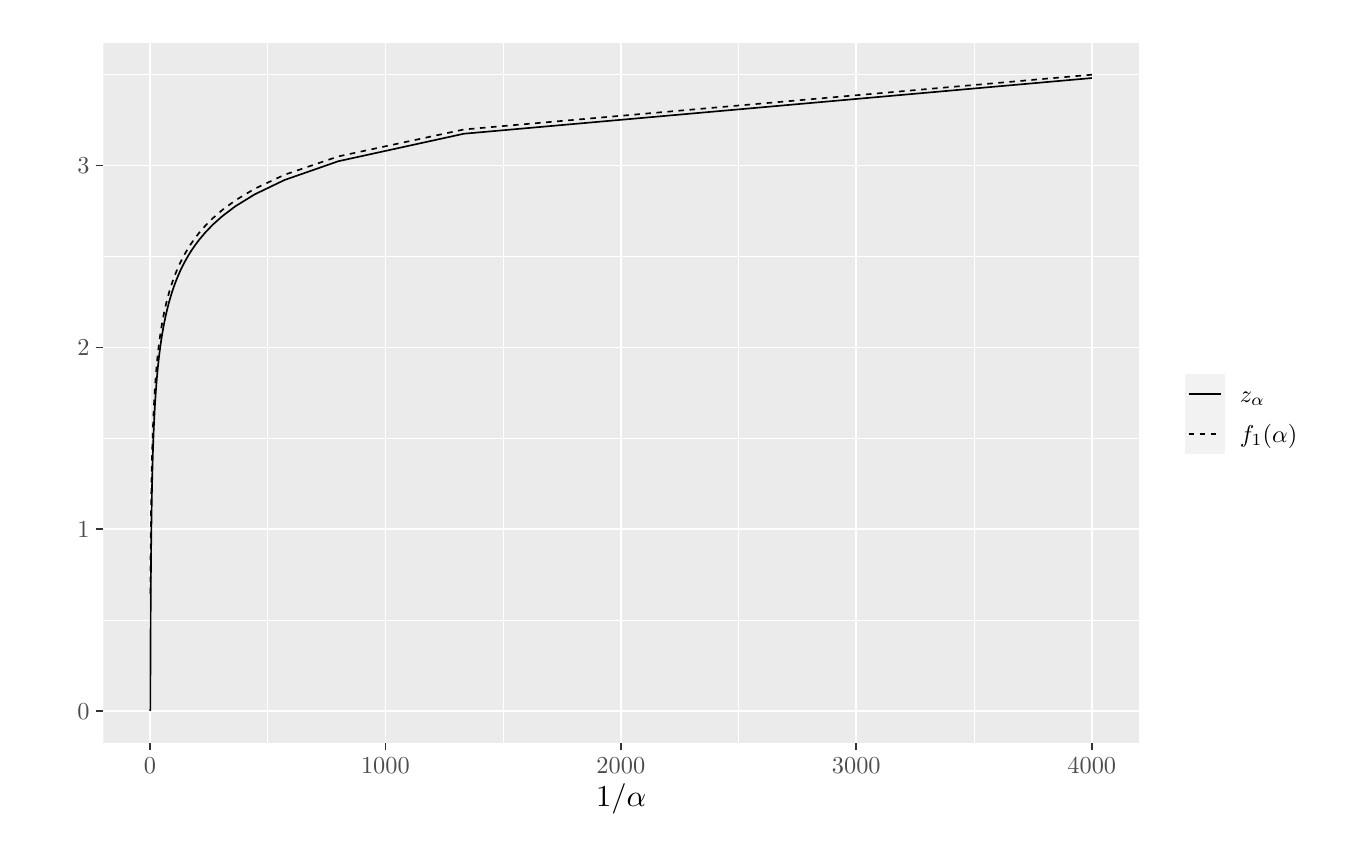
\begin{tikzpicture}[x=1pt,y=1pt]
\definecolor{fillColor}{RGB}{255,255,255}
\path[use as bounding box,fill=fillColor,fill opacity=0.00] (0,0) rectangle (469.75,289.08);
\begin{scope}
\path[clip] (  0.00,  0.00) rectangle (469.75,289.08);
\definecolor{drawColor}{RGB}{255,255,255}
\definecolor{fillColor}{RGB}{255,255,255}

\path[draw=drawColor,line width= 0.6pt,line join=round,line cap=round,fill=fillColor] (  0.00,  0.00) rectangle (469.76,289.08);
\end{scope}
\begin{scope}
\path[clip] ( 27.31, 30.69) rectangle (401.54,283.58);
\definecolor{fillColor}{gray}{0.92}

\path[fill=fillColor] ( 27.31, 30.69) rectangle (401.54,283.58);
\definecolor{drawColor}{RGB}{255,255,255}

\path[draw=drawColor,line width= 0.3pt,line join=round] ( 27.31, 75.00) --
	(401.54, 75.00);

\path[draw=drawColor,line width= 0.3pt,line join=round] ( 27.31,140.71) --
	(401.54,140.71);

\path[draw=drawColor,line width= 0.3pt,line join=round] ( 27.31,206.42) --
	(401.54,206.42);

\path[draw=drawColor,line width= 0.3pt,line join=round] ( 27.31,272.13) --
	(401.54,272.13);

\path[draw=drawColor,line width= 0.3pt,line join=round] ( 86.70, 30.69) --
	( 86.70,283.58);

\path[draw=drawColor,line width= 0.3pt,line join=round] (171.79, 30.69) --
	(171.79,283.58);

\path[draw=drawColor,line width= 0.3pt,line join=round] (256.89, 30.69) --
	(256.89,283.58);

\path[draw=drawColor,line width= 0.3pt,line join=round] (341.98, 30.69) --
	(341.98,283.58);

\path[draw=drawColor,line width= 0.6pt,line join=round] ( 27.31, 42.14) --
	(401.54, 42.14);

\path[draw=drawColor,line width= 0.6pt,line join=round] ( 27.31,107.85) --
	(401.54,107.85);

\path[draw=drawColor,line width= 0.6pt,line join=round] ( 27.31,173.56) --
	(401.54,173.56);

\path[draw=drawColor,line width= 0.6pt,line join=round] ( 27.31,239.27) --
	(401.54,239.27);

\path[draw=drawColor,line width= 0.6pt,line join=round] ( 44.15, 30.69) --
	( 44.15,283.58);

\path[draw=drawColor,line width= 0.6pt,line join=round] (129.25, 30.69) --
	(129.25,283.58);

\path[draw=drawColor,line width= 0.6pt,line join=round] (214.34, 30.69) --
	(214.34,283.58);

\path[draw=drawColor,line width= 0.6pt,line join=round] (299.43, 30.69) --
	(299.43,283.58);

\path[draw=drawColor,line width= 0.6pt,line join=round] (384.53, 30.69) --
	(384.53,283.58);
\definecolor{drawColor}{RGB}{0,0,0}

\path[draw=drawColor,line width= 0.6pt,line join=round] ( 44.32, 42.18) --
	( 44.32, 42.26) --
	( 44.32, 42.35) --
	( 44.32, 42.43) --
	( 44.32, 42.51) --
	( 44.32, 42.59) --
	( 44.32, 42.68) --
	( 44.32, 42.76) --
	( 44.32, 42.84) --
	( 44.33, 42.92) --
	( 44.33, 43.00) --
	( 44.33, 43.09) --
	( 44.33, 43.17) --
	( 44.33, 43.25) --
	( 44.33, 43.33) --
	( 44.33, 43.42) --
	( 44.33, 43.50) --
	( 44.33, 43.58) --
	( 44.33, 43.66) --
	( 44.33, 43.75) --
	( 44.33, 43.83) --
	( 44.33, 43.91) --
	( 44.33, 43.99) --
	( 44.33, 44.08) --
	( 44.33, 44.16) --
	( 44.33, 44.24) --
	( 44.33, 44.32) --
	( 44.33, 44.41) --
	( 44.33, 44.49) --
	( 44.33, 44.57) --
	( 44.33, 44.65) --
	( 44.33, 44.73) --
	( 44.33, 44.82) --
	( 44.33, 44.90) --
	( 44.33, 44.98) --
	( 44.33, 45.06) --
	( 44.33, 45.15) --
	( 44.33, 45.23) --
	( 44.33, 45.31) --
	( 44.33, 45.39) --
	( 44.33, 45.48) --
	( 44.33, 45.56) --
	( 44.33, 45.64) --
	( 44.33, 45.72) --
	( 44.33, 45.81) --
	( 44.33, 45.89) --
	( 44.33, 45.97) --
	( 44.33, 46.05) --
	( 44.33, 46.14) --
	( 44.33, 46.22) --
	( 44.33, 46.30) --
	( 44.33, 46.38) --
	( 44.33, 46.47) --
	( 44.33, 46.55) --
	( 44.33, 46.63) --
	( 44.33, 46.71) --
	( 44.33, 46.80) --
	( 44.33, 46.88) --
	( 44.33, 46.96) --
	( 44.33, 47.04) --
	( 44.33, 47.13) --
	( 44.33, 47.21) --
	( 44.33, 47.29) --
	( 44.33, 47.38) --
	( 44.34, 47.46) --
	( 44.34, 47.54) --
	( 44.34, 47.62) --
	( 44.34, 47.71) --
	( 44.34, 47.79) --
	( 44.34, 47.87) --
	( 44.34, 47.95) --
	( 44.34, 48.04) --
	( 44.34, 48.12) --
	( 44.34, 48.20) --
	( 44.34, 48.28) --
	( 44.34, 48.37) --
	( 44.34, 48.45) --
	( 44.34, 48.53) --
	( 44.34, 48.62) --
	( 44.34, 48.70) --
	( 44.34, 48.78) --
	( 44.34, 48.86) --
	( 44.34, 48.95) --
	( 44.34, 49.03) --
	( 44.34, 49.11) --
	( 44.34, 49.19) --
	( 44.34, 49.28) --
	( 44.34, 49.36) --
	( 44.34, 49.44) --
	( 44.34, 49.53) --
	( 44.34, 49.61) --
	( 44.34, 49.69) --
	( 44.34, 49.78) --
	( 44.34, 49.86) --
	( 44.34, 49.94) --
	( 44.34, 50.02) --
	( 44.34, 50.11) --
	( 44.34, 50.19) --
	( 44.34, 50.27) --
	( 44.34, 50.36) --
	( 44.34, 50.44) --
	( 44.34, 50.52) --
	( 44.34, 50.60) --
	( 44.34, 50.69) --
	( 44.34, 50.77) --
	( 44.34, 50.85) --
	( 44.34, 50.94) --
	( 44.34, 51.02) --
	( 44.34, 51.10) --
	( 44.34, 51.19) --
	( 44.34, 51.27) --
	( 44.34, 51.35) --
	( 44.34, 51.44) --
	( 44.35, 51.52) --
	( 44.35, 51.60) --
	( 44.35, 51.69) --
	( 44.35, 51.77) --
	( 44.35, 51.85) --
	( 44.35, 51.94) --
	( 44.35, 52.02) --
	( 44.35, 52.10) --
	( 44.35, 52.19) --
	( 44.35, 52.27) --
	( 44.35, 52.35) --
	( 44.35, 52.44) --
	( 44.35, 52.52) --
	( 44.35, 52.60) --
	( 44.35, 52.69) --
	( 44.35, 52.77) --
	( 44.35, 52.85) --
	( 44.35, 52.94) --
	( 44.35, 53.02) --
	( 44.35, 53.10) --
	( 44.35, 53.19) --
	( 44.35, 53.27) --
	( 44.35, 53.35) --
	( 44.35, 53.44) --
	( 44.35, 53.52) --
	( 44.35, 53.60) --
	( 44.35, 53.69) --
	( 44.35, 53.77) --
	( 44.35, 53.86) --
	( 44.35, 53.94) --
	( 44.35, 54.02) --
	( 44.35, 54.11) --
	( 44.35, 54.19) --
	( 44.35, 54.27) --
	( 44.35, 54.36) --
	( 44.35, 54.44) --
	( 44.35, 54.53) --
	( 44.35, 54.61) --
	( 44.35, 54.69) --
	( 44.35, 54.78) --
	( 44.35, 54.86) --
	( 44.35, 54.94) --
	( 44.35, 55.03) --
	( 44.35, 55.11) --
	( 44.36, 55.20) --
	( 44.36, 55.28) --
	( 44.36, 55.36) --
	( 44.36, 55.45) --
	( 44.36, 55.53) --
	( 44.36, 55.62) --
	( 44.36, 55.70) --
	( 44.36, 55.79) --
	( 44.36, 55.87) --
	( 44.36, 55.95) --
	( 44.36, 56.04) --
	( 44.36, 56.12) --
	( 44.36, 56.21) --
	( 44.36, 56.29) --
	( 44.36, 56.37) --
	( 44.36, 56.46) --
	( 44.36, 56.54) --
	( 44.36, 56.63) --
	( 44.36, 56.71) --
	( 44.36, 56.80) --
	( 44.36, 56.88) --
	( 44.36, 56.97) --
	( 44.36, 57.05) --
	( 44.36, 57.13) --
	( 44.36, 57.22) --
	( 44.36, 57.30) --
	( 44.36, 57.39) --
	( 44.36, 57.47) --
	( 44.36, 57.56) --
	( 44.36, 57.64) --
	( 44.36, 57.73) --
	( 44.36, 57.81) --
	( 44.36, 57.90) --
	( 44.36, 57.98) --
	( 44.36, 58.07) --
	( 44.36, 58.15) --
	( 44.36, 58.24) --
	( 44.36, 58.32) --
	( 44.36, 58.41) --
	( 44.37, 58.49) --
	( 44.37, 58.58) --
	( 44.37, 58.66) --
	( 44.37, 58.75) --
	( 44.37, 58.83) --
	( 44.37, 58.92) --
	( 44.37, 59.00) --
	( 44.37, 59.09) --
	( 44.37, 59.17) --
	( 44.37, 59.26) --
	( 44.37, 59.34) --
	( 44.37, 59.43) --
	( 44.37, 59.51) --
	( 44.37, 59.60) --
	( 44.37, 59.68) --
	( 44.37, 59.77) --
	( 44.37, 59.85) --
	( 44.37, 59.94) --
	( 44.37, 60.02) --
	( 44.37, 60.11) --
	( 44.37, 60.19) --
	( 44.37, 60.28) --
	( 44.37, 60.37) --
	( 44.37, 60.45) --
	( 44.37, 60.54) --
	( 44.37, 60.62) --
	( 44.37, 60.71) --
	( 44.37, 60.79) --
	( 44.37, 60.88) --
	( 44.37, 60.97) --
	( 44.37, 61.05) --
	( 44.37, 61.14) --
	( 44.37, 61.22) --
	( 44.37, 61.31) --
	( 44.37, 61.40) --
	( 44.37, 61.48) --
	( 44.37, 61.57) --
	( 44.38, 61.65) --
	( 44.38, 61.74) --
	( 44.38, 61.83) --
	( 44.38, 61.91) --
	( 44.38, 62.00) --
	( 44.38, 62.08) --
	( 44.38, 62.17) --
	( 44.38, 62.26) --
	( 44.38, 62.34) --
	( 44.38, 62.43) --
	( 44.38, 62.52) --
	( 44.38, 62.60) --
	( 44.38, 62.69) --
	( 44.38, 62.78) --
	( 44.38, 62.86) --
	( 44.38, 62.95) --
	( 44.38, 63.03) --
	( 44.38, 63.12) --
	( 44.38, 63.21) --
	( 44.38, 63.29) --
	( 44.38, 63.38) --
	( 44.38, 63.47) --
	( 44.38, 63.56) --
	( 44.38, 63.64) --
	( 44.38, 63.73) --
	( 44.38, 63.82) --
	( 44.38, 63.90) --
	( 44.38, 63.99) --
	( 44.38, 64.08) --
	( 44.38, 64.16) --
	( 44.38, 64.25) --
	( 44.38, 64.34) --
	( 44.38, 64.43) --
	( 44.39, 64.51) --
	( 44.39, 64.60) --
	( 44.39, 64.69) --
	( 44.39, 64.77) --
	( 44.39, 64.86) --
	( 44.39, 64.95) --
	( 44.39, 65.04) --
	( 44.39, 65.12) --
	( 44.39, 65.21) --
	( 44.39, 65.30) --
	( 44.39, 65.39) --
	( 44.39, 65.48) --
	( 44.39, 65.56) --
	( 44.39, 65.65) --
	( 44.39, 65.74) --
	( 44.39, 65.83) --
	( 44.39, 65.91) --
	( 44.39, 66.00) --
	( 44.39, 66.09) --
	( 44.39, 66.18) --
	( 44.39, 66.27) --
	( 44.39, 66.35) --
	( 44.39, 66.44) --
	( 44.39, 66.53) --
	( 44.39, 66.62) --
	( 44.39, 66.71) --
	( 44.39, 66.80) --
	( 44.39, 66.88) --
	( 44.39, 66.97) --
	( 44.39, 67.06) --
	( 44.40, 67.15) --
	( 44.40, 67.24) --
	( 44.40, 67.33) --
	( 44.40, 67.42) --
	( 44.40, 67.50) --
	( 44.40, 67.59) --
	( 44.40, 67.68) --
	( 44.40, 67.77) --
	( 44.40, 67.86) --
	( 44.40, 67.95) --
	( 44.40, 68.04) --
	( 44.40, 68.13) --
	( 44.40, 68.22) --
	( 44.40, 68.30) --
	( 44.40, 68.39) --
	( 44.40, 68.48) --
	( 44.40, 68.57) --
	( 44.40, 68.66) --
	( 44.40, 68.75) --
	( 44.40, 68.84) --
	( 44.40, 68.93) --
	( 44.40, 69.02) --
	( 44.40, 69.11) --
	( 44.40, 69.20) --
	( 44.40, 69.29) --
	( 44.40, 69.38) --
	( 44.40, 69.47) --
	( 44.40, 69.56) --
	( 44.41, 69.65) --
	( 44.41, 69.74) --
	( 44.41, 69.83) --
	( 44.41, 69.92) --
	( 44.41, 70.01) --
	( 44.41, 70.10) --
	( 44.41, 70.19) --
	( 44.41, 70.28) --
	( 44.41, 70.37) --
	( 44.41, 70.46) --
	( 44.41, 70.55) --
	( 44.41, 70.64) --
	( 44.41, 70.73) --
	( 44.41, 70.82) --
	( 44.41, 70.91) --
	( 44.41, 71.00) --
	( 44.41, 71.09) --
	( 44.41, 71.18) --
	( 44.41, 71.27) --
	( 44.41, 71.37) --
	( 44.41, 71.46) --
	( 44.41, 71.55) --
	( 44.41, 71.64) --
	( 44.41, 71.73) --
	( 44.41, 71.82) --
	( 44.41, 71.91) --
	( 44.42, 72.00) --
	( 44.42, 72.09) --
	( 44.42, 72.19) --
	( 44.42, 72.28) --
	( 44.42, 72.37) --
	( 44.42, 72.46) --
	( 44.42, 72.55) --
	( 44.42, 72.64) --
	( 44.42, 72.74) --
	( 44.42, 72.83) --
	( 44.42, 72.92) --
	( 44.42, 73.01) --
	( 44.42, 73.10) --
	( 44.42, 73.20) --
	( 44.42, 73.29) --
	( 44.42, 73.38) --
	( 44.42, 73.47) --
	( 44.42, 73.56) --
	( 44.42, 73.66) --
	( 44.42, 73.75) --
	( 44.42, 73.84) --
	( 44.42, 73.93) --
	( 44.42, 74.03) --
	( 44.42, 74.12) --
	( 44.43, 74.21) --
	( 44.43, 74.30) --
	( 44.43, 74.40) --
	( 44.43, 74.49) --
	( 44.43, 74.58) --
	( 44.43, 74.68) --
	( 44.43, 74.77) --
	( 44.43, 74.86) --
	( 44.43, 74.96) --
	( 44.43, 75.05) --
	( 44.43, 75.14) --
	( 44.43, 75.24) --
	( 44.43, 75.33) --
	( 44.43, 75.42) --
	( 44.43, 75.52) --
	( 44.43, 75.61) --
	( 44.43, 75.70) --
	( 44.43, 75.80) --
	( 44.43, 75.89) --
	( 44.43, 75.99) --
	( 44.43, 76.08) --
	( 44.43, 76.17) --
	( 44.44, 76.27) --
	( 44.44, 76.36) --
	( 44.44, 76.46) --
	( 44.44, 76.55) --
	( 44.44, 76.65) --
	( 44.44, 76.74) --
	( 44.44, 76.84) --
	( 44.44, 76.93) --
	( 44.44, 77.03) --
	( 44.44, 77.12) --
	( 44.44, 77.21) --
	( 44.44, 77.31) --
	( 44.44, 77.40) --
	( 44.44, 77.50) --
	( 44.44, 77.60) --
	( 44.44, 77.69) --
	( 44.44, 77.79) --
	( 44.44, 77.88) --
	( 44.44, 77.98) --
	( 44.44, 78.07) --
	( 44.44, 78.17) --
	( 44.45, 78.26) --
	( 44.45, 78.36) --
	( 44.45, 78.46) --
	( 44.45, 78.55) --
	( 44.45, 78.65) --
	( 44.45, 78.74) --
	( 44.45, 78.84) --
	( 44.45, 78.94) --
	( 44.45, 79.03) --
	( 44.45, 79.13) --
	( 44.45, 79.23) --
	( 44.45, 79.32) --
	( 44.45, 79.42) --
	( 44.45, 79.52) --
	( 44.45, 79.61) --
	( 44.45, 79.71) --
	( 44.45, 79.81) --
	( 44.45, 79.90) --
	( 44.45, 80.00) --
	( 44.46, 80.10) --
	( 44.46, 80.20) --
	( 44.46, 80.29) --
	( 44.46, 80.39) --
	( 44.46, 80.49) --
	( 44.46, 80.59) --
	( 44.46, 80.68) --
	( 44.46, 80.78) --
	( 44.46, 80.88) --
	( 44.46, 80.98) --
	( 44.46, 81.08) --
	( 44.46, 81.17) --
	( 44.46, 81.27) --
	( 44.46, 81.37) --
	( 44.46, 81.47) --
	( 44.46, 81.57) --
	( 44.46, 81.67) --
	( 44.46, 81.76) --
	( 44.47, 81.86) --
	( 44.47, 81.96) --
	( 44.47, 82.06) --
	( 44.47, 82.16) --
	( 44.47, 82.26) --
	( 44.47, 82.36) --
	( 44.47, 82.46) --
	( 44.47, 82.56) --
	( 44.47, 82.66) --
	( 44.47, 82.76) --
	( 44.47, 82.86) --
	( 44.47, 82.96) --
	( 44.47, 83.06) --
	( 44.47, 83.16) --
	( 44.47, 83.26) --
	( 44.47, 83.36) --
	( 44.47, 83.46) --
	( 44.48, 83.56) --
	( 44.48, 83.66) --
	( 44.48, 83.76) --
	( 44.48, 83.86) --
	( 44.48, 83.96) --
	( 44.48, 84.06) --
	( 44.48, 84.16) --
	( 44.48, 84.26) --
	( 44.48, 84.36) --
	( 44.48, 84.47) --
	( 44.48, 84.57) --
	( 44.48, 84.67) --
	( 44.48, 84.77) --
	( 44.48, 84.87) --
	( 44.48, 84.97) --
	( 44.48, 85.08) --
	( 44.49, 85.18) --
	( 44.49, 85.28) --
	( 44.49, 85.38) --
	( 44.49, 85.48) --
	( 44.49, 85.59) --
	( 44.49, 85.69) --
	( 44.49, 85.79) --
	( 44.49, 85.89) --
	( 44.49, 86.00) --
	( 44.49, 86.10) --
	( 44.49, 86.20) --
	( 44.49, 86.31) --
	( 44.49, 86.41) --
	( 44.49, 86.51) --
	( 44.49, 86.62) --
	( 44.50, 86.72) --
	( 44.50, 86.82) --
	( 44.50, 86.93) --
	( 44.50, 87.03) --
	( 44.50, 87.14) --
	( 44.50, 87.24) --
	( 44.50, 87.34) --
	( 44.50, 87.45) --
	( 44.50, 87.55) --
	( 44.50, 87.66) --
	( 44.50, 87.76) --
	( 44.50, 87.87) --
	( 44.50, 87.97) --
	( 44.50, 88.08) --
	( 44.51, 88.18) --
	( 44.51, 88.29) --
	( 44.51, 88.39) --
	( 44.51, 88.50) --
	( 44.51, 88.61) --
	( 44.51, 88.71) --
	( 44.51, 88.82) --
	( 44.51, 88.92) --
	( 44.51, 89.03) --
	( 44.51, 89.14) --
	( 44.51, 89.24) --
	( 44.51, 89.35) --
	( 44.51, 89.45) --
	( 44.51, 89.56) --
	( 44.52, 89.67) --
	( 44.52, 89.78) --
	( 44.52, 89.88) --
	( 44.52, 89.99) --
	( 44.52, 90.10) --
	( 44.52, 90.21) --
	( 44.52, 90.31) --
	( 44.52, 90.42) --
	( 44.52, 90.53) --
	( 44.52, 90.64) --
	( 44.52, 90.74) --
	( 44.52, 90.85) --
	( 44.53, 90.96) --
	( 44.53, 91.07) --
	( 44.53, 91.18) --
	( 44.53, 91.29) --
	( 44.53, 91.40) --
	( 44.53, 91.51) --
	( 44.53, 91.62) --
	( 44.53, 91.72) --
	( 44.53, 91.83) --
	( 44.53, 91.94) --
	( 44.53, 92.05) --
	( 44.53, 92.16) --
	( 44.54, 92.27) --
	( 44.54, 92.38) --
	( 44.54, 92.49) --
	( 44.54, 92.61) --
	( 44.54, 92.72) --
	( 44.54, 92.83) --
	( 44.54, 92.94) --
	( 44.54, 93.05) --
	( 44.54, 93.16) --
	( 44.54, 93.27) --
	( 44.54, 93.38) --
	( 44.54, 93.49) --
	( 44.55, 93.61) --
	( 44.55, 93.72) --
	( 44.55, 93.83) --
	( 44.55, 93.94) --
	( 44.55, 94.06) --
	( 44.55, 94.17) --
	( 44.55, 94.28) --
	( 44.55, 94.39) --
	( 44.55, 94.51) --
	( 44.55, 94.62) --
	( 44.56, 94.73) --
	( 44.56, 94.85) --
	( 44.56, 94.96) --
	( 44.56, 95.07) --
	( 44.56, 95.19) --
	( 44.56, 95.30) --
	( 44.56, 95.42) --
	( 44.56, 95.53) --
	( 44.56, 95.65) --
	( 44.56, 95.76) --
	( 44.56, 95.88) --
	( 44.57, 95.99) --
	( 44.57, 96.11) --
	( 44.57, 96.22) --
	( 44.57, 96.34) --
	( 44.57, 96.45) --
	( 44.57, 96.57) --
	( 44.57, 96.69) --
	( 44.57, 96.80) --
	( 44.57, 96.92) --
	( 44.58, 97.03) --
	( 44.58, 97.15) --
	( 44.58, 97.27) --
	( 44.58, 97.39) --
	( 44.58, 97.50) --
	( 44.58, 97.62) --
	( 44.58, 97.74) --
	( 44.58, 97.86) --
	( 44.58, 97.97) --
	( 44.58, 98.09) --
	( 44.59, 98.21) --
	( 44.59, 98.33) --
	( 44.59, 98.45) --
	( 44.59, 98.57) --
	( 44.59, 98.69) --
	( 44.59, 98.81) --
	( 44.59, 98.93) --
	( 44.59, 99.04) --
	( 44.59, 99.16) --
	( 44.60, 99.29) --
	( 44.60, 99.41) --
	( 44.60, 99.53) --
	( 44.60, 99.65) --
	( 44.60, 99.77) --
	( 44.60, 99.89) --
	( 44.60,100.01) --
	( 44.60,100.13) --
	( 44.61,100.25) --
	( 44.61,100.37) --
	( 44.61,100.50) --
	( 44.61,100.62) --
	( 44.61,100.74) --
	( 44.61,100.86) --
	( 44.61,100.99) --
	( 44.61,101.11) --
	( 44.62,101.23) --
	( 44.62,101.36) --
	( 44.62,101.48) --
	( 44.62,101.60) --
	( 44.62,101.73) --
	( 44.62,101.85) --
	( 44.62,101.98) --
	( 44.62,102.10) --
	( 44.63,102.23) --
	( 44.63,102.35) --
	( 44.63,102.48) --
	( 44.63,102.60) --
	( 44.63,102.73) --
	( 44.63,102.86) --
	( 44.63,102.98) --
	( 44.63,103.11) --
	( 44.64,103.24) --
	( 44.64,103.36) --
	( 44.64,103.49) --
	( 44.64,103.62) --
	( 44.64,103.74) --
	( 44.64,103.87) --
	( 44.64,104.00) --
	( 44.65,104.13) --
	( 44.65,104.26) --
	( 44.65,104.39) --
	( 44.65,104.52) --
	( 44.65,104.65) --
	( 44.65,104.77) --
	( 44.65,104.90) --
	( 44.66,105.03) --
	( 44.66,105.17) --
	( 44.66,105.30) --
	( 44.66,105.43) --
	( 44.66,105.56) --
	( 44.66,105.69) --
	( 44.67,105.82) --
	( 44.67,105.95) --
	( 44.67,106.08) --
	( 44.67,106.22) --
	( 44.67,106.35) --
	( 44.67,106.48) --
	( 44.67,106.62) --
	( 44.68,106.75) --
	( 44.68,106.88) --
	( 44.68,107.02) --
	( 44.68,107.15) --
	( 44.68,107.29) --
	( 44.68,107.42) --
	( 44.69,107.55) --
	( 44.69,107.69) --
	( 44.69,107.83) --
	( 44.69,107.96) --
	( 44.69,108.10) --
	( 44.69,108.23) --
	( 44.70,108.37) --
	( 44.70,108.51) --
	( 44.70,108.65) --
	( 44.70,108.78) --
	( 44.70,108.92) --
	( 44.70,109.06) --
	( 44.71,109.20) --
	( 44.71,109.34) --
	( 44.71,109.48) --
	( 44.71,109.61) --
	( 44.71,109.75) --
	( 44.72,109.89) --
	( 44.72,110.03) --
	( 44.72,110.18) --
	( 44.72,110.32) --
	( 44.72,110.46) --
	( 44.73,110.60) --
	( 44.73,110.74) --
	( 44.73,110.88) --
	( 44.73,111.03) --
	( 44.73,111.17) --
	( 44.74,111.31) --
	( 44.74,111.45) --
	( 44.74,111.60) --
	( 44.74,111.74) --
	( 44.74,111.89) --
	( 44.75,112.03) --
	( 44.75,112.18) --
	( 44.75,112.32) --
	( 44.75,112.47) --
	( 44.75,112.61) --
	( 44.76,112.76) --
	( 44.76,112.91) --
	( 44.76,113.06) --
	( 44.76,113.20) --
	( 44.76,113.35) --
	( 44.77,113.50) --
	( 44.77,113.65) --
	( 44.77,113.80) --
	( 44.77,113.95) --
	( 44.78,114.10) --
	( 44.78,114.25) --
	( 44.78,114.40) --
	( 44.78,114.55) --
	( 44.78,114.70) --
	( 44.79,114.85) --
	( 44.79,115.00) --
	( 44.79,115.16) --
	( 44.79,115.31) --
	( 44.80,115.46) --
	( 44.80,115.62) --
	( 44.80,115.77) --
	( 44.80,115.92) --
	( 44.81,116.08) --
	( 44.81,116.23) --
	( 44.81,116.39) --
	( 44.81,116.55) --
	( 44.82,116.70) --
	( 44.82,116.86) --
	( 44.82,117.02) --
	( 44.82,117.18) --
	( 44.83,117.33) --
	( 44.83,117.49) --
	( 44.83,117.65) --
	( 44.84,117.81) --
	( 44.84,117.97) --
	( 44.84,118.13) --
	( 44.84,118.29) --
	( 44.85,118.45) --
	( 44.85,118.62) --
	( 44.85,118.78) --
	( 44.86,118.94) --
	( 44.86,119.10) --
	( 44.86,119.27) --
	( 44.86,119.43) --
	( 44.87,119.60) --
	( 44.87,119.76) --
	( 44.87,119.93) --
	( 44.88,120.09) --
	( 44.88,120.26) --
	( 44.88,120.43) --
	( 44.89,120.60) --
	( 44.89,120.76) --
	( 44.89,120.93) --
	( 44.89,121.10) --
	( 44.90,121.27) --
	( 44.90,121.44) --
	( 44.90,121.61) --
	( 44.91,121.78) --
	( 44.91,121.96) --
	( 44.91,122.13) --
	( 44.92,122.30) --
	( 44.92,122.48) --
	( 44.93,122.65) --
	( 44.93,122.82) --
	( 44.93,123.00) --
	( 44.94,123.18) --
	( 44.94,123.35) --
	( 44.94,123.53) --
	( 44.95,123.71) --
	( 44.95,123.89) --
	( 44.95,124.06) --
	( 44.96,124.24) --
	( 44.96,124.42) --
	( 44.97,124.60) --
	( 44.97,124.79) --
	( 44.97,124.97) --
	( 44.98,125.15) --
	( 44.98,125.33) --
	( 44.99,125.52) --
	( 44.99,125.70) --
	( 44.99,125.89) --
	( 45.00,126.07) --
	( 45.00,126.26) --
	( 45.01,126.45) --
	( 45.01,126.63) --
	( 45.01,126.82) --
	( 45.02,127.01) --
	( 45.02,127.20) --
	( 45.03,127.39) --
	( 45.03,127.58) --
	( 45.04,127.78) --
	( 45.04,127.97) --
	( 45.05,128.16) --
	( 45.05,128.36) --
	( 45.06,128.55) --
	( 45.06,128.75) --
	( 45.07,128.95) --
	( 45.07,129.14) --
	( 45.08,129.34) --
	( 45.08,129.54) --
	( 45.09,129.74) --
	( 45.09,129.94) --
	( 45.10,130.14) --
	( 45.10,130.34) --
	( 45.11,130.55) --
	( 45.11,130.75) --
	( 45.12,130.96) --
	( 45.12,131.16) --
	( 45.13,131.37) --
	( 45.13,131.58) --
	( 45.14,131.78) --
	( 45.15,131.99) --
	( 45.15,132.20) --
	( 45.16,132.42) --
	( 45.16,132.63) --
	( 45.17,132.84) --
	( 45.18,133.05) --
	( 45.18,133.27) --
	( 45.19,133.49) --
	( 45.19,133.70) --
	( 45.20,133.92) --
	( 45.21,134.14) --
	( 45.21,134.36) --
	( 45.22,134.58) --
	( 45.23,134.80) --
	( 45.23,135.03) --
	( 45.24,135.25) --
	( 45.25,135.47) --
	( 45.25,135.70) --
	( 45.26,135.93) --
	( 45.27,136.16) --
	( 45.28,136.39) --
	( 45.28,136.62) --
	( 45.29,136.85) --
	( 45.30,137.08) --
	( 45.31,137.32) --
	( 45.31,137.55) --
	( 45.32,137.79) --
	( 45.33,138.03) --
	( 45.34,138.27) --
	( 45.35,138.51) --
	( 45.36,138.75) --
	( 45.36,138.99) --
	( 45.37,139.24) --
	( 45.38,139.49) --
	( 45.39,139.73) --
	( 45.40,139.98) --
	( 45.41,140.23) --
	( 45.42,140.48) --
	( 45.43,140.74) --
	( 45.44,140.99) --
	( 45.45,141.25) --
	( 45.46,141.50) --
	( 45.47,141.76) --
	( 45.48,142.02) --
	( 45.49,142.29) --
	( 45.50,142.55) --
	( 45.51,142.82) --
	( 45.52,143.08) --
	( 45.53,143.35) --
	( 45.54,143.62) --
	( 45.55,143.89) --
	( 45.57,144.17) --
	( 45.58,144.44) --
	( 45.59,144.72) --
	( 45.60,145.00) --
	( 45.61,145.28) --
	( 45.63,145.57) --
	( 45.64,145.85) --
	( 45.65,146.14) --
	( 45.67,146.43) --
	( 45.68,146.72) --
	( 45.69,147.01) --
	( 45.71,147.31) --
	( 45.72,147.61) --
	( 45.74,147.90) --
	( 45.75,148.21) --
	( 45.77,148.51) --
	( 45.78,148.82) --
	( 45.80,149.13) --
	( 45.81,149.44) --
	( 45.83,149.75) --
	( 45.85,150.07) --
	( 45.86,150.39) --
	( 45.88,150.71) --
	( 45.90,151.03) --
	( 45.92,151.36) --
	( 45.94,151.69) --
	( 45.95,152.02) --
	( 45.97,152.35) --
	( 45.99,152.69) --
	( 46.01,153.03) --
	( 46.03,153.37) --
	( 46.05,153.72) --
	( 46.08,154.07) --
	( 46.10,154.42) --
	( 46.12,154.78) --
	( 46.14,155.14) --
	( 46.17,155.50) --
	( 46.19,155.87) --
	( 46.22,156.24) --
	( 46.24,156.61) --
	( 46.27,156.99) --
	( 46.29,157.37) --
	( 46.32,157.76) --
	( 46.35,158.15) --
	( 46.38,158.54) --
	( 46.41,158.94) --
	( 46.44,159.34) --
	( 46.47,159.74) --
	( 46.50,160.16) --
	( 46.53,160.57) --
	( 46.57,160.99) --
	( 46.60,161.42) --
	( 46.64,161.85) --
	( 46.67,162.28) --
	( 46.71,162.72) --
	( 46.75,163.17) --
	( 46.79,163.62) --
	( 46.83,164.08) --
	( 46.88,164.54) --
	( 46.92,165.01) --
	( 46.97,165.49) --
	( 47.01,165.97) --
	( 47.06,166.46) --
	( 47.11,166.96) --
	( 47.17,167.46) --
	( 47.22,167.97) --
	( 47.28,168.49) --
	( 47.33,169.02) --
	( 47.39,169.56) --
	( 47.46,170.10) --
	( 47.52,170.65) --
	( 47.59,171.21) --
	( 47.66,171.79) --
	( 47.74,172.37) --
	( 47.81,172.96) --
	( 47.89,173.56) --
	( 47.98,174.18) --
	( 48.07,174.80) --
	( 48.16,175.44) --
	( 48.25,176.09) --
	( 48.36,176.76) --
	( 48.46,177.44) --
	( 48.57,178.13) --
	( 48.69,178.84) --
	( 48.82,179.56) --
	( 48.95,180.31) --
	( 49.09,181.07) --
	( 49.23,181.85) --
	( 49.39,182.65) --
	( 49.56,183.47) --
	( 49.73,184.31) --
	( 49.92,185.18) --
	( 50.12,186.07) --
	( 50.34,186.99) --
	( 50.58,187.94) --
	( 50.83,188.92) --
	( 51.10,189.94) --
	( 51.40,190.99) --
	( 51.72,192.08) --
	( 52.07,193.22) --
	( 52.46,194.40) --
	( 52.88,195.63) --
	( 53.35,196.92) --
	( 53.88,198.27) --
	( 54.47,199.69) --
	( 55.13,201.19) --
	( 55.89,202.78) --
	( 56.76,204.47) --
	( 57.77,206.27) --
	( 58.95,208.20) --
	( 60.36,210.29) --
	( 62.07,212.56) --
	( 64.18,215.06) --
	( 66.84,217.84) --
	( 70.34,220.97) --
	( 75.10,224.57) --
	( 81.97,228.81) --
	( 92.78,234.02) --
	(112.23,240.81) --
	(157.61,250.75) --
	(384.53,270.87);

\path[draw=drawColor,line width= 0.6pt,dash pattern=on 2pt off 2pt ,line join=round] ( 44.32, 84.68) --
	( 44.32, 84.71) --
	( 44.32, 84.74) --
	( 44.32, 84.77) --
	( 44.32, 84.80) --
	( 44.32, 84.83) --
	( 44.32, 84.86) --
	( 44.32, 84.89) --
	( 44.32, 84.92) --
	( 44.33, 84.95) --
	( 44.33, 84.98) --
	( 44.33, 85.01) --
	( 44.33, 85.04) --
	( 44.33, 85.07) --
	( 44.33, 85.10) --
	( 44.33, 85.13) --
	( 44.33, 85.16) --
	( 44.33, 85.20) --
	( 44.33, 85.23) --
	( 44.33, 85.26) --
	( 44.33, 85.29) --
	( 44.33, 85.32) --
	( 44.33, 85.35) --
	( 44.33, 85.38) --
	( 44.33, 85.41) --
	( 44.33, 85.44) --
	( 44.33, 85.47) --
	( 44.33, 85.50) --
	( 44.33, 85.53) --
	( 44.33, 85.57) --
	( 44.33, 85.60) --
	( 44.33, 85.63) --
	( 44.33, 85.66) --
	( 44.33, 85.69) --
	( 44.33, 85.72) --
	( 44.33, 85.75) --
	( 44.33, 85.79) --
	( 44.33, 85.82) --
	( 44.33, 85.85) --
	( 44.33, 85.88) --
	( 44.33, 85.91) --
	( 44.33, 85.94) --
	( 44.33, 85.97) --
	( 44.33, 86.01) --
	( 44.33, 86.04) --
	( 44.33, 86.07) --
	( 44.33, 86.10) --
	( 44.33, 86.13) --
	( 44.33, 86.17) --
	( 44.33, 86.20) --
	( 44.33, 86.23) --
	( 44.33, 86.26) --
	( 44.33, 86.29) --
	( 44.33, 86.33) --
	( 44.33, 86.36) --
	( 44.33, 86.39) --
	( 44.33, 86.42) --
	( 44.33, 86.45) --
	( 44.33, 86.49) --
	( 44.33, 86.52) --
	( 44.33, 86.55) --
	( 44.33, 86.58) --
	( 44.33, 86.62) --
	( 44.33, 86.65) --
	( 44.34, 86.68) --
	( 44.34, 86.71) --
	( 44.34, 86.75) --
	( 44.34, 86.78) --
	( 44.34, 86.81) --
	( 44.34, 86.85) --
	( 44.34, 86.88) --
	( 44.34, 86.91) --
	( 44.34, 86.94) --
	( 44.34, 86.98) --
	( 44.34, 87.01) --
	( 44.34, 87.04) --
	( 44.34, 87.08) --
	( 44.34, 87.11) --
	( 44.34, 87.14) --
	( 44.34, 87.18) --
	( 44.34, 87.21) --
	( 44.34, 87.24) --
	( 44.34, 87.28) --
	( 44.34, 87.31) --
	( 44.34, 87.34) --
	( 44.34, 87.38) --
	( 44.34, 87.41) --
	( 44.34, 87.44) --
	( 44.34, 87.48) --
	( 44.34, 87.51) --
	( 44.34, 87.54) --
	( 44.34, 87.58) --
	( 44.34, 87.61) --
	( 44.34, 87.65) --
	( 44.34, 87.68) --
	( 44.34, 87.71) --
	( 44.34, 87.75) --
	( 44.34, 87.78) --
	( 44.34, 87.82) --
	( 44.34, 87.85) --
	( 44.34, 87.89) --
	( 44.34, 87.92) --
	( 44.34, 87.95) --
	( 44.34, 87.99) --
	( 44.34, 88.02) --
	( 44.34, 88.06) --
	( 44.34, 88.09) --
	( 44.34, 88.13) --
	( 44.34, 88.16) --
	( 44.34, 88.20) --
	( 44.34, 88.23) --
	( 44.34, 88.26) --
	( 44.34, 88.30) --
	( 44.35, 88.33) --
	( 44.35, 88.37) --
	( 44.35, 88.40) --
	( 44.35, 88.44) --
	( 44.35, 88.47) --
	( 44.35, 88.51) --
	( 44.35, 88.54) --
	( 44.35, 88.58) --
	( 44.35, 88.61) --
	( 44.35, 88.65) --
	( 44.35, 88.69) --
	( 44.35, 88.72) --
	( 44.35, 88.76) --
	( 44.35, 88.79) --
	( 44.35, 88.83) --
	( 44.35, 88.86) --
	( 44.35, 88.90) --
	( 44.35, 88.93) --
	( 44.35, 88.97) --
	( 44.35, 89.01) --
	( 44.35, 89.04) --
	( 44.35, 89.08) --
	( 44.35, 89.11) --
	( 44.35, 89.15) --
	( 44.35, 89.19) --
	( 44.35, 89.22) --
	( 44.35, 89.26) --
	( 44.35, 89.29) --
	( 44.35, 89.33) --
	( 44.35, 89.37) --
	( 44.35, 89.40) --
	( 44.35, 89.44) --
	( 44.35, 89.48) --
	( 44.35, 89.51) --
	( 44.35, 89.55) --
	( 44.35, 89.59) --
	( 44.35, 89.62) --
	( 44.35, 89.66) --
	( 44.35, 89.70) --
	( 44.35, 89.73) --
	( 44.35, 89.77) --
	( 44.35, 89.81) --
	( 44.35, 89.84) --
	( 44.35, 89.88) --
	( 44.36, 89.92) --
	( 44.36, 89.95) --
	( 44.36, 89.99) --
	( 44.36, 90.03) --
	( 44.36, 90.07) --
	( 44.36, 90.10) --
	( 44.36, 90.14) --
	( 44.36, 90.18) --
	( 44.36, 90.22) --
	( 44.36, 90.25) --
	( 44.36, 90.29) --
	( 44.36, 90.33) --
	( 44.36, 90.37) --
	( 44.36, 90.40) --
	( 44.36, 90.44) --
	( 44.36, 90.48) --
	( 44.36, 90.52) --
	( 44.36, 90.56) --
	( 44.36, 90.59) --
	( 44.36, 90.63) --
	( 44.36, 90.67) --
	( 44.36, 90.71) --
	( 44.36, 90.75) --
	( 44.36, 90.78) --
	( 44.36, 90.82) --
	( 44.36, 90.86) --
	( 44.36, 90.90) --
	( 44.36, 90.94) --
	( 44.36, 90.98) --
	( 44.36, 91.02) --
	( 44.36, 91.05) --
	( 44.36, 91.09) --
	( 44.36, 91.13) --
	( 44.36, 91.17) --
	( 44.36, 91.21) --
	( 44.36, 91.25) --
	( 44.36, 91.29) --
	( 44.36, 91.33) --
	( 44.36, 91.37) --
	( 44.37, 91.41) --
	( 44.37, 91.44) --
	( 44.37, 91.48) --
	( 44.37, 91.52) --
	( 44.37, 91.56) --
	( 44.37, 91.60) --
	( 44.37, 91.64) --
	( 44.37, 91.68) --
	( 44.37, 91.72) --
	( 44.37, 91.76) --
	( 44.37, 91.80) --
	( 44.37, 91.84) --
	( 44.37, 91.88) --
	( 44.37, 91.92) --
	( 44.37, 91.96) --
	( 44.37, 92.00) --
	( 44.37, 92.04) --
	( 44.37, 92.08) --
	( 44.37, 92.12) --
	( 44.37, 92.16) --
	( 44.37, 92.20) --
	( 44.37, 92.24) --
	( 44.37, 92.28) --
	( 44.37, 92.32) --
	( 44.37, 92.36) --
	( 44.37, 92.40) --
	( 44.37, 92.45) --
	( 44.37, 92.49) --
	( 44.37, 92.53) --
	( 44.37, 92.57) --
	( 44.37, 92.61) --
	( 44.37, 92.65) --
	( 44.37, 92.69) --
	( 44.37, 92.73) --
	( 44.37, 92.77) --
	( 44.37, 92.82) --
	( 44.37, 92.86) --
	( 44.38, 92.90) --
	( 44.38, 92.94) --
	( 44.38, 92.98) --
	( 44.38, 93.02) --
	( 44.38, 93.06) --
	( 44.38, 93.11) --
	( 44.38, 93.15) --
	( 44.38, 93.19) --
	( 44.38, 93.23) --
	( 44.38, 93.27) --
	( 44.38, 93.32) --
	( 44.38, 93.36) --
	( 44.38, 93.40) --
	( 44.38, 93.44) --
	( 44.38, 93.48) --
	( 44.38, 93.53) --
	( 44.38, 93.57) --
	( 44.38, 93.61) --
	( 44.38, 93.65) --
	( 44.38, 93.70) --
	( 44.38, 93.74) --
	( 44.38, 93.78) --
	( 44.38, 93.83) --
	( 44.38, 93.87) --
	( 44.38, 93.91) --
	( 44.38, 93.95) --
	( 44.38, 94.00) --
	( 44.38, 94.04) --
	( 44.38, 94.08) --
	( 44.38, 94.13) --
	( 44.38, 94.17) --
	( 44.38, 94.21) --
	( 44.38, 94.26) --
	( 44.39, 94.30) --
	( 44.39, 94.35) --
	( 44.39, 94.39) --
	( 44.39, 94.43) --
	( 44.39, 94.48) --
	( 44.39, 94.52) --
	( 44.39, 94.56) --
	( 44.39, 94.61) --
	( 44.39, 94.65) --
	( 44.39, 94.70) --
	( 44.39, 94.74) --
	( 44.39, 94.79) --
	( 44.39, 94.83) --
	( 44.39, 94.87) --
	( 44.39, 94.92) --
	( 44.39, 94.96) --
	( 44.39, 95.01) --
	( 44.39, 95.05) --
	( 44.39, 95.10) --
	( 44.39, 95.14) --
	( 44.39, 95.19) --
	( 44.39, 95.23) --
	( 44.39, 95.28) --
	( 44.39, 95.32) --
	( 44.39, 95.37) --
	( 44.39, 95.41) --
	( 44.39, 95.46) --
	( 44.39, 95.50) --
	( 44.39, 95.55) --
	( 44.39, 95.60) --
	( 44.40, 95.64) --
	( 44.40, 95.69) --
	( 44.40, 95.73) --
	( 44.40, 95.78) --
	( 44.40, 95.83) --
	( 44.40, 95.87) --
	( 44.40, 95.92) --
	( 44.40, 95.96) --
	( 44.40, 96.01) --
	( 44.40, 96.06) --
	( 44.40, 96.10) --
	( 44.40, 96.15) --
	( 44.40, 96.20) --
	( 44.40, 96.24) --
	( 44.40, 96.29) --
	( 44.40, 96.34) --
	( 44.40, 96.38) --
	( 44.40, 96.43) --
	( 44.40, 96.48) --
	( 44.40, 96.52) --
	( 44.40, 96.57) --
	( 44.40, 96.62) --
	( 44.40, 96.67) --
	( 44.40, 96.71) --
	( 44.40, 96.76) --
	( 44.40, 96.81) --
	( 44.40, 96.86) --
	( 44.40, 96.90) --
	( 44.41, 96.95) --
	( 44.41, 97.00) --
	( 44.41, 97.05) --
	( 44.41, 97.10) --
	( 44.41, 97.14) --
	( 44.41, 97.19) --
	( 44.41, 97.24) --
	( 44.41, 97.29) --
	( 44.41, 97.34) --
	( 44.41, 97.39) --
	( 44.41, 97.43) --
	( 44.41, 97.48) --
	( 44.41, 97.53) --
	( 44.41, 97.58) --
	( 44.41, 97.63) --
	( 44.41, 97.68) --
	( 44.41, 97.73) --
	( 44.41, 97.78) --
	( 44.41, 97.83) --
	( 44.41, 97.88) --
	( 44.41, 97.92) --
	( 44.41, 97.97) --
	( 44.41, 98.02) --
	( 44.41, 98.07) --
	( 44.41, 98.12) --
	( 44.41, 98.17) --
	( 44.42, 98.22) --
	( 44.42, 98.27) --
	( 44.42, 98.32) --
	( 44.42, 98.37) --
	( 44.42, 98.42) --
	( 44.42, 98.47) --
	( 44.42, 98.52) --
	( 44.42, 98.57) --
	( 44.42, 98.63) --
	( 44.42, 98.68) --
	( 44.42, 98.73) --
	( 44.42, 98.78) --
	( 44.42, 98.83) --
	( 44.42, 98.88) --
	( 44.42, 98.93) --
	( 44.42, 98.98) --
	( 44.42, 99.03) --
	( 44.42, 99.08) --
	( 44.42, 99.14) --
	( 44.42, 99.19) --
	( 44.42, 99.24) --
	( 44.42, 99.29) --
	( 44.42, 99.34) --
	( 44.42, 99.39) --
	( 44.43, 99.45) --
	( 44.43, 99.50) --
	( 44.43, 99.55) --
	( 44.43, 99.60) --
	( 44.43, 99.66) --
	( 44.43, 99.71) --
	( 44.43, 99.76) --
	( 44.43, 99.81) --
	( 44.43, 99.87) --
	( 44.43, 99.92) --
	( 44.43, 99.97) --
	( 44.43,100.02) --
	( 44.43,100.08) --
	( 44.43,100.13) --
	( 44.43,100.18) --
	( 44.43,100.24) --
	( 44.43,100.29) --
	( 44.43,100.34) --
	( 44.43,100.40) --
	( 44.43,100.45) --
	( 44.43,100.51) --
	( 44.43,100.56) --
	( 44.44,100.61) --
	( 44.44,100.67) --
	( 44.44,100.72) --
	( 44.44,100.78) --
	( 44.44,100.83) --
	( 44.44,100.89) --
	( 44.44,100.94) --
	( 44.44,100.99) --
	( 44.44,101.05) --
	( 44.44,101.10) --
	( 44.44,101.16) --
	( 44.44,101.21) --
	( 44.44,101.27) --
	( 44.44,101.32) --
	( 44.44,101.38) --
	( 44.44,101.44) --
	( 44.44,101.49) --
	( 44.44,101.55) --
	( 44.44,101.60) --
	( 44.44,101.66) --
	( 44.44,101.71) --
	( 44.45,101.77) --
	( 44.45,101.83) --
	( 44.45,101.88) --
	( 44.45,101.94) --
	( 44.45,102.00) --
	( 44.45,102.05) --
	( 44.45,102.11) --
	( 44.45,102.17) --
	( 44.45,102.22) --
	( 44.45,102.28) --
	( 44.45,102.34) --
	( 44.45,102.39) --
	( 44.45,102.45) --
	( 44.45,102.51) --
	( 44.45,102.57) --
	( 44.45,102.62) --
	( 44.45,102.68) --
	( 44.45,102.74) --
	( 44.45,102.80) --
	( 44.46,102.86) --
	( 44.46,102.91) --
	( 44.46,102.97) --
	( 44.46,103.03) --
	( 44.46,103.09) --
	( 44.46,103.15) --
	( 44.46,103.21) --
	( 44.46,103.27) --
	( 44.46,103.32) --
	( 44.46,103.38) --
	( 44.46,103.44) --
	( 44.46,103.50) --
	( 44.46,103.56) --
	( 44.46,103.62) --
	( 44.46,103.68) --
	( 44.46,103.74) --
	( 44.46,103.80) --
	( 44.46,103.86) --
	( 44.47,103.92) --
	( 44.47,103.98) --
	( 44.47,104.04) --
	( 44.47,104.10) --
	( 44.47,104.16) --
	( 44.47,104.22) --
	( 44.47,104.28) --
	( 44.47,104.34) --
	( 44.47,104.40) --
	( 44.47,104.47) --
	( 44.47,104.53) --
	( 44.47,104.59) --
	( 44.47,104.65) --
	( 44.47,104.71) --
	( 44.47,104.77) --
	( 44.47,104.83) --
	( 44.47,104.90) --
	( 44.48,104.96) --
	( 44.48,105.02) --
	( 44.48,105.08) --
	( 44.48,105.15) --
	( 44.48,105.21) --
	( 44.48,105.27) --
	( 44.48,105.33) --
	( 44.48,105.40) --
	( 44.48,105.46) --
	( 44.48,105.52) --
	( 44.48,105.59) --
	( 44.48,105.65) --
	( 44.48,105.71) --
	( 44.48,105.78) --
	( 44.48,105.84) --
	( 44.48,105.90) --
	( 44.49,105.97) --
	( 44.49,106.03) --
	( 44.49,106.10) --
	( 44.49,106.16) --
	( 44.49,106.23) --
	( 44.49,106.29) --
	( 44.49,106.35) --
	( 44.49,106.42) --
	( 44.49,106.48) --
	( 44.49,106.55) --
	( 44.49,106.62) --
	( 44.49,106.68) --
	( 44.49,106.75) --
	( 44.49,106.81) --
	( 44.49,106.88) --
	( 44.50,106.94) --
	( 44.50,107.01) --
	( 44.50,107.08) --
	( 44.50,107.14) --
	( 44.50,107.21) --
	( 44.50,107.28) --
	( 44.50,107.34) --
	( 44.50,107.41) --
	( 44.50,107.48) --
	( 44.50,107.54) --
	( 44.50,107.61) --
	( 44.50,107.68) --
	( 44.50,107.75) --
	( 44.50,107.81) --
	( 44.51,107.88) --
	( 44.51,107.95) --
	( 44.51,108.02) --
	( 44.51,108.09) --
	( 44.51,108.15) --
	( 44.51,108.22) --
	( 44.51,108.29) --
	( 44.51,108.36) --
	( 44.51,108.43) --
	( 44.51,108.50) --
	( 44.51,108.57) --
	( 44.51,108.64) --
	( 44.51,108.71) --
	( 44.51,108.78) --
	( 44.52,108.85) --
	( 44.52,108.92) --
	( 44.52,108.99) --
	( 44.52,109.06) --
	( 44.52,109.13) --
	( 44.52,109.20) --
	( 44.52,109.27) --
	( 44.52,109.34) --
	( 44.52,109.41) --
	( 44.52,109.48) --
	( 44.52,109.55) --
	( 44.52,109.63) --
	( 44.53,109.70) --
	( 44.53,109.77) --
	( 44.53,109.84) --
	( 44.53,109.91) --
	( 44.53,109.99) --
	( 44.53,110.06) --
	( 44.53,110.13) --
	( 44.53,110.20) --
	( 44.53,110.28) --
	( 44.53,110.35) --
	( 44.53,110.42) --
	( 44.53,110.50) --
	( 44.54,110.57) --
	( 44.54,110.64) --
	( 44.54,110.72) --
	( 44.54,110.79) --
	( 44.54,110.87) --
	( 44.54,110.94) --
	( 44.54,111.02) --
	( 44.54,111.09) --
	( 44.54,111.16) --
	( 44.54,111.24) --
	( 44.54,111.32) --
	( 44.54,111.39) --
	( 44.55,111.47) --
	( 44.55,111.54) --
	( 44.55,111.62) --
	( 44.55,111.69) --
	( 44.55,111.77) --
	( 44.55,111.85) --
	( 44.55,111.92) --
	( 44.55,112.00) --
	( 44.55,112.08) --
	( 44.55,112.15) --
	( 44.56,112.23) --
	( 44.56,112.31) --
	( 44.56,112.39) --
	( 44.56,112.46) --
	( 44.56,112.54) --
	( 44.56,112.62) --
	( 44.56,112.70) --
	( 44.56,112.78) --
	( 44.56,112.86) --
	( 44.56,112.94) --
	( 44.56,113.01) --
	( 44.57,113.09) --
	( 44.57,113.17) --
	( 44.57,113.25) --
	( 44.57,113.33) --
	( 44.57,113.41) --
	( 44.57,113.49) --
	( 44.57,113.57) --
	( 44.57,113.65) --
	( 44.57,113.74) --
	( 44.58,113.82) --
	( 44.58,113.90) --
	( 44.58,113.98) --
	( 44.58,114.06) --
	( 44.58,114.14) --
	( 44.58,114.22) --
	( 44.58,114.31) --
	( 44.58,114.39) --
	( 44.58,114.47) --
	( 44.58,114.55) --
	( 44.59,114.64) --
	( 44.59,114.72) --
	( 44.59,114.80) --
	( 44.59,114.89) --
	( 44.59,114.97) --
	( 44.59,115.06) --
	( 44.59,115.14) --
	( 44.59,115.22) --
	( 44.59,115.31) --
	( 44.60,115.39) --
	( 44.60,115.48) --
	( 44.60,115.56) --
	( 44.60,115.65) --
	( 44.60,115.74) --
	( 44.60,115.82) --
	( 44.60,115.91) --
	( 44.60,115.99) --
	( 44.61,116.08) --
	( 44.61,116.17) --
	( 44.61,116.25) --
	( 44.61,116.34) --
	( 44.61,116.43) --
	( 44.61,116.52) --
	( 44.61,116.60) --
	( 44.61,116.69) --
	( 44.62,116.78) --
	( 44.62,116.87) --
	( 44.62,116.96) --
	( 44.62,117.05) --
	( 44.62,117.14) --
	( 44.62,117.23) --
	( 44.62,117.32) --
	( 44.62,117.41) --
	( 44.63,117.50) --
	( 44.63,117.59) --
	( 44.63,117.68) --
	( 44.63,117.77) --
	( 44.63,117.86) --
	( 44.63,117.95) --
	( 44.63,118.04) --
	( 44.63,118.13) --
	( 44.64,118.23) --
	( 44.64,118.32) --
	( 44.64,118.41) --
	( 44.64,118.50) --
	( 44.64,118.60) --
	( 44.64,118.69) --
	( 44.64,118.78) --
	( 44.65,118.88) --
	( 44.65,118.97) --
	( 44.65,119.07) --
	( 44.65,119.16) --
	( 44.65,119.25) --
	( 44.65,119.35) --
	( 44.65,119.45) --
	( 44.66,119.54) --
	( 44.66,119.64) --
	( 44.66,119.73) --
	( 44.66,119.83) --
	( 44.66,119.93) --
	( 44.66,120.02) --
	( 44.67,120.12) --
	( 44.67,120.22) --
	( 44.67,120.32) --
	( 44.67,120.41) --
	( 44.67,120.51) --
	( 44.67,120.61) --
	( 44.67,120.71) --
	( 44.68,120.81) --
	( 44.68,120.91) --
	( 44.68,121.01) --
	( 44.68,121.11) --
	( 44.68,121.21) --
	( 44.68,121.31) --
	( 44.69,121.41) --
	( 44.69,121.51) --
	( 44.69,121.61) --
	( 44.69,121.71) --
	( 44.69,121.82) --
	( 44.69,121.92) --
	( 44.70,122.02) --
	( 44.70,122.12) --
	( 44.70,122.23) --
	( 44.70,122.33) --
	( 44.70,122.44) --
	( 44.70,122.54) --
	( 44.71,122.64) --
	( 44.71,122.75) --
	( 44.71,122.85) --
	( 44.71,122.96) --
	( 44.71,123.07) --
	( 44.72,123.17) --
	( 44.72,123.28) --
	( 44.72,123.38) --
	( 44.72,123.49) --
	( 44.72,123.60) --
	( 44.73,123.71) --
	( 44.73,123.82) --
	( 44.73,123.92) --
	( 44.73,124.03) --
	( 44.73,124.14) --
	( 44.74,124.25) --
	( 44.74,124.36) --
	( 44.74,124.47) --
	( 44.74,124.58) --
	( 44.74,124.69) --
	( 44.75,124.80) --
	( 44.75,124.91) --
	( 44.75,125.03) --
	( 44.75,125.14) --
	( 44.75,125.25) --
	( 44.76,125.36) --
	( 44.76,125.48) --
	( 44.76,125.59) --
	( 44.76,125.71) --
	( 44.76,125.82) --
	( 44.77,125.93) --
	( 44.77,126.05) --
	( 44.77,126.17) --
	( 44.77,126.28) --
	( 44.78,126.40) --
	( 44.78,126.51) --
	( 44.78,126.63) --
	( 44.78,126.75) --
	( 44.78,126.87) --
	( 44.79,126.98) --
	( 44.79,127.10) --
	( 44.79,127.22) --
	( 44.79,127.34) --
	( 44.80,127.46) --
	( 44.80,127.58) --
	( 44.80,127.70) --
	( 44.80,127.82) --
	( 44.81,127.95) --
	( 44.81,128.07) --
	( 44.81,128.19) --
	( 44.81,128.31) --
	( 44.82,128.44) --
	( 44.82,128.56) --
	( 44.82,128.68) --
	( 44.82,128.81) --
	( 44.83,128.93) --
	( 44.83,129.06) --
	( 44.83,129.19) --
	( 44.84,129.31) --
	( 44.84,129.44) --
	( 44.84,129.57) --
	( 44.84,129.69) --
	( 44.85,129.82) --
	( 44.85,129.95) --
	( 44.85,130.08) --
	( 44.86,130.21) --
	( 44.86,130.34) --
	( 44.86,130.47) --
	( 44.86,130.60) --
	( 44.87,130.73) --
	( 44.87,130.86) --
	( 44.87,131.00) --
	( 44.88,131.13) --
	( 44.88,131.26) --
	( 44.88,131.40) --
	( 44.89,131.53) --
	( 44.89,131.67) --
	( 44.89,131.80) --
	( 44.89,131.94) --
	( 44.90,132.08) --
	( 44.90,132.21) --
	( 44.90,132.35) --
	( 44.91,132.49) --
	( 44.91,132.63) --
	( 44.91,132.77) --
	( 44.92,132.91) --
	( 44.92,133.05) --
	( 44.93,133.19) --
	( 44.93,133.33) --
	( 44.93,133.47) --
	( 44.94,133.62) --
	( 44.94,133.76) --
	( 44.94,133.90) --
	( 44.95,134.05) --
	( 44.95,134.19) --
	( 44.95,134.34) --
	( 44.96,134.49) --
	( 44.96,134.63) --
	( 44.97,134.78) --
	( 44.97,134.93) --
	( 44.97,135.08) --
	( 44.98,135.23) --
	( 44.98,135.38) --
	( 44.99,135.53) --
	( 44.99,135.68) --
	( 44.99,135.83) --
	( 45.00,135.99) --
	( 45.00,136.14) --
	( 45.01,136.29) --
	( 45.01,136.45) --
	( 45.01,136.60) --
	( 45.02,136.76) --
	( 45.02,136.92) --
	( 45.03,137.08) --
	( 45.03,137.23) --
	( 45.04,137.39) --
	( 45.04,137.55) --
	( 45.05,137.71) --
	( 45.05,137.87) --
	( 45.06,138.04) --
	( 45.06,138.20) --
	( 45.07,138.36) --
	( 45.07,138.53) --
	( 45.08,138.69) --
	( 45.08,138.86) --
	( 45.09,139.03) --
	( 45.09,139.19) --
	( 45.10,139.36) --
	( 45.10,139.53) --
	( 45.11,139.70) --
	( 45.11,139.87) --
	( 45.12,140.04) --
	( 45.12,140.22) --
	( 45.13,140.39) --
	( 45.13,140.57) --
	( 45.14,140.74) --
	( 45.15,140.92) --
	( 45.15,141.09) --
	( 45.16,141.27) --
	( 45.16,141.45) --
	( 45.17,141.63) --
	( 45.18,141.81) --
	( 45.18,141.99) --
	( 45.19,142.18) --
	( 45.19,142.36) --
	( 45.20,142.55) --
	( 45.21,142.73) --
	( 45.21,142.92) --
	( 45.22,143.11) --
	( 45.23,143.29) --
	( 45.23,143.48) --
	( 45.24,143.68) --
	( 45.25,143.87) --
	( 45.25,144.06) --
	( 45.26,144.26) --
	( 45.27,144.45) --
	( 45.28,144.65) --
	( 45.28,144.84) --
	( 45.29,145.04) --
	( 45.30,145.24) --
	( 45.31,145.44) --
	( 45.31,145.65) --
	( 45.32,145.85) --
	( 45.33,146.06) --
	( 45.34,146.26) --
	( 45.35,146.47) --
	( 45.36,146.68) --
	( 45.36,146.89) --
	( 45.37,147.10) --
	( 45.38,147.31) --
	( 45.39,147.52) --
	( 45.40,147.74) --
	( 45.41,147.96) --
	( 45.42,148.17) --
	( 45.43,148.39) --
	( 45.44,148.61) --
	( 45.45,148.84) --
	( 45.46,149.06) --
	( 45.47,149.29) --
	( 45.48,149.51) --
	( 45.49,149.74) --
	( 45.50,149.97) --
	( 45.51,150.20) --
	( 45.52,150.44) --
	( 45.53,150.67) --
	( 45.54,150.91) --
	( 45.55,151.15) --
	( 45.57,151.39) --
	( 45.58,151.63) --
	( 45.59,151.87) --
	( 45.60,152.12) --
	( 45.61,152.36) --
	( 45.63,152.61) --
	( 45.64,152.86) --
	( 45.65,153.12) --
	( 45.67,153.37) --
	( 45.68,153.63) --
	( 45.69,153.89) --
	( 45.71,154.15) --
	( 45.72,154.41) --
	( 45.74,154.68) --
	( 45.75,154.94) --
	( 45.77,155.21) --
	( 45.78,155.49) --
	( 45.80,155.76) --
	( 45.81,156.04) --
	( 45.83,156.31) --
	( 45.85,156.60) --
	( 45.86,156.88) --
	( 45.88,157.16) --
	( 45.90,157.45) --
	( 45.92,157.74) --
	( 45.94,158.04) --
	( 45.95,158.34) --
	( 45.97,158.63) --
	( 45.99,158.94) --
	( 46.01,159.24) --
	( 46.03,159.55) --
	( 46.05,159.86) --
	( 46.08,160.17) --
	( 46.10,160.49) --
	( 46.12,160.81) --
	( 46.14,161.14) --
	( 46.17,161.46) --
	( 46.19,161.79) --
	( 46.22,162.13) --
	( 46.24,162.46) --
	( 46.27,162.81) --
	( 46.29,163.15) --
	( 46.32,163.50) --
	( 46.35,163.85) --
	( 46.38,164.21) --
	( 46.41,164.57) --
	( 46.44,164.93) --
	( 46.47,165.30) --
	( 46.50,165.68) --
	( 46.53,166.05) --
	( 46.57,166.44) --
	( 46.60,166.82) --
	( 46.64,167.22) --
	( 46.67,167.61) --
	( 46.71,168.02) --
	( 46.75,168.42) --
	( 46.79,168.84) --
	( 46.83,169.26) --
	( 46.88,169.68) --
	( 46.92,170.11) --
	( 46.97,170.55) --
	( 47.01,170.99) --
	( 47.06,171.44) --
	( 47.11,171.90) --
	( 47.17,172.37) --
	( 47.22,172.84) --
	( 47.28,173.32) --
	( 47.33,173.80) --
	( 47.39,174.30) --
	( 47.46,174.80) --
	( 47.52,175.31) --
	( 47.59,175.83) --
	( 47.66,176.36) --
	( 47.74,176.90) --
	( 47.81,177.45) --
	( 47.89,178.02) --
	( 47.98,178.59) --
	( 48.07,179.17) --
	( 48.16,179.76) --
	( 48.25,180.37) --
	( 48.36,180.99) --
	( 48.46,181.63) --
	( 48.57,182.28) --
	( 48.69,182.94) --
	( 48.82,183.62) --
	( 48.95,184.32) --
	( 49.09,185.03) --
	( 49.23,185.76) --
	( 49.39,186.51) --
	( 49.56,187.29) --
	( 49.73,188.08) --
	( 49.92,188.90) --
	( 50.12,189.74) --
	( 50.34,190.61) --
	( 50.58,191.51) --
	( 50.83,192.44) --
	( 51.10,193.41) --
	( 51.40,194.40) --
	( 51.72,195.44) --
	( 52.07,196.52) --
	( 52.46,197.65) --
	( 52.88,198.82) --
	( 53.35,200.05) --
	( 53.88,201.34) --
	( 54.47,202.70) --
	( 55.13,204.14) --
	( 55.89,205.66) --
	( 56.76,207.28) --
	( 57.77,209.01) --
	( 58.95,210.87) --
	( 60.36,212.88) --
	( 62.07,215.08) --
	( 64.18,217.49) --
	( 66.84,220.18) --
	( 70.34,223.21) --
	( 75.10,226.71) --
	( 81.97,230.84) --
	( 92.78,235.91) --
	(112.23,242.55) --
	(157.61,252.29) --
	(384.53,272.08);
\end{scope}
\begin{scope}
\path[clip] (  0.00,  0.00) rectangle (469.75,289.08);
\definecolor{drawColor}{gray}{0.30}

\node[text=drawColor,anchor=base east,inner sep=0pt, outer sep=0pt, scale=  0.88] at ( 22.36, 39.11) {0};

\node[text=drawColor,anchor=base east,inner sep=0pt, outer sep=0pt, scale=  0.88] at ( 22.36,104.82) {1};

\node[text=drawColor,anchor=base east,inner sep=0pt, outer sep=0pt, scale=  0.88] at ( 22.36,170.53) {2};

\node[text=drawColor,anchor=base east,inner sep=0pt, outer sep=0pt, scale=  0.88] at ( 22.36,236.24) {3};
\end{scope}
\begin{scope}
\path[clip] (  0.00,  0.00) rectangle (469.75,289.08);
\definecolor{drawColor}{gray}{0.20}

\path[draw=drawColor,line width= 0.6pt,line join=round] ( 24.56, 42.14) --
	( 27.31, 42.14);

\path[draw=drawColor,line width= 0.6pt,line join=round] ( 24.56,107.85) --
	( 27.31,107.85);

\path[draw=drawColor,line width= 0.6pt,line join=round] ( 24.56,173.56) --
	( 27.31,173.56);

\path[draw=drawColor,line width= 0.6pt,line join=round] ( 24.56,239.27) --
	( 27.31,239.27);
\end{scope}
\begin{scope}
\path[clip] (  0.00,  0.00) rectangle (469.75,289.08);
\definecolor{drawColor}{gray}{0.20}

\path[draw=drawColor,line width= 0.6pt,line join=round] ( 44.15, 27.94) --
	( 44.15, 30.69);

\path[draw=drawColor,line width= 0.6pt,line join=round] (129.25, 27.94) --
	(129.25, 30.69);

\path[draw=drawColor,line width= 0.6pt,line join=round] (214.34, 27.94) --
	(214.34, 30.69);

\path[draw=drawColor,line width= 0.6pt,line join=round] (299.43, 27.94) --
	(299.43, 30.69);

\path[draw=drawColor,line width= 0.6pt,line join=round] (384.53, 27.94) --
	(384.53, 30.69);
\end{scope}
\begin{scope}
\path[clip] (  0.00,  0.00) rectangle (469.75,289.08);
\definecolor{drawColor}{gray}{0.30}

\node[text=drawColor,anchor=base,inner sep=0pt, outer sep=0pt, scale=  0.88] at ( 44.15, 19.68) {0};

\node[text=drawColor,anchor=base,inner sep=0pt, outer sep=0pt, scale=  0.88] at (129.25, 19.68) {1000};

\node[text=drawColor,anchor=base,inner sep=0pt, outer sep=0pt, scale=  0.88] at (214.34, 19.68) {2000};

\node[text=drawColor,anchor=base,inner sep=0pt, outer sep=0pt, scale=  0.88] at (299.43, 19.68) {3000};

\node[text=drawColor,anchor=base,inner sep=0pt, outer sep=0pt, scale=  0.88] at (384.53, 19.68) {4000};
\end{scope}
\begin{scope}
\path[clip] (  0.00,  0.00) rectangle (469.75,289.08);
\definecolor{drawColor}{RGB}{0,0,0}

\node[text=drawColor,anchor=base,inner sep=0pt, outer sep=0pt, scale=  1.10] at (214.43,  7.64) {$1 / \alpha$};
\end{scope}
\begin{scope}
\path[clip] (  0.00,  0.00) rectangle (469.75,289.08);
\definecolor{fillColor}{RGB}{255,255,255}

\path[fill=fillColor] (412.54,129.57) rectangle (464.25,184.69);
\end{scope}
\begin{scope}
\path[clip] (  0.00,  0.00) rectangle (469.75,289.08);
\definecolor{fillColor}{gray}{0.95}

\path[fill=fillColor] (418.04,149.53) rectangle (432.49,163.98);
\end{scope}
\begin{scope}
\path[clip] (  0.00,  0.00) rectangle (469.75,289.08);
\definecolor{drawColor}{RGB}{0,0,0}

\path[draw=drawColor,line width= 0.6pt,line join=round] (419.48,156.75) -- (431.05,156.75);
\end{scope}
\begin{scope}
\path[clip] (  0.00,  0.00) rectangle (469.75,289.08);
\definecolor{fillColor}{gray}{0.95}

\path[fill=fillColor] (418.04,135.07) rectangle (432.49,149.53);
\end{scope}
\begin{scope}
\path[clip] (  0.00,  0.00) rectangle (469.75,289.08);
\definecolor{drawColor}{RGB}{0,0,0}

\path[draw=drawColor,line width= 0.6pt,dash pattern=on 2pt off 2pt ,line join=round] (419.48,142.30) -- (431.05,142.30);
\end{scope}
\begin{scope}
\path[clip] (  0.00,  0.00) rectangle (469.75,289.08);
\definecolor{drawColor}{RGB}{0,0,0}

\node[text=drawColor,anchor=base west,inner sep=0pt, outer sep=0pt, scale=  0.88] at (437.99,153.72) {$z_\alpha$};
\end{scope}
\begin{scope}
\path[clip] (  0.00,  0.00) rectangle (469.75,289.08);
\definecolor{drawColor}{RGB}{0,0,0}

\node[text=drawColor,anchor=base west,inner sep=0pt, outer sep=0pt, scale=  0.88] at (437.99,139.27) {$f_1(\alpha)$};
\end{scope}
\end{tikzpicture}

\caption{The Gaussian quantile function and the direct upper bound plotted as functions of $1 / \alpha$}.
\label{fig_bound}
\end{figure}

While we have the shown that the direct upper bound is asymptotically tight, this does not address its use as a numerical approximation of $z_a$.  Figure~\ref{fig_bound} shows $z_\alpha$ and $f_1(\alpha)$ plotted as functions of $1 / \alpha$, and it clearly shows that there is a large difference even when $\alpha = \maxAlpha$.  This difference is approximately $\maxAlphaDiff$, which suggests that the convergence in Theorem~\ref{thm_tight_diff} is too slow for $f_1(\alpha)$ to be treated as a reasonable numerical approximation of $z_\alpha$.

\section{Strongly Consistent Interval Estimates}
\label{sec_conf_int}

We will now use the Gaussian quantile inequalities we have proved to construct strongly consistent interval estimates for an unknown population mean.  Before we do so, however, we will comment on the definition of strong consistency.  In what follows, given an interval $I$ we will write $\ell(I)$, $r(I)$ and $|I|$ to respectively denote its left endpoint, its right endpoint, and its length.  All of the convergence properties we discuss will be in the large sample limit.

In~\cite{rising2023orderPersp}, a sequence of interval estimates $\hat{I}_n$ was said to be \emph{strongly consistent} for a parameter $\theta$ if the sequences $\ell(\hat{I}_n)$ and $r(\hat{I}_n)$ are both consistent point estimates of $\theta$ and $\prob{\theta \in \hat{I}_n}$ converges to $1$.  We will state and prove an equivalent definition in Theorem~\ref{thm_def_equiv}.

\begin{theorem}
\label{thm_def_equiv}
A sequence of interval estimates $\hat{I}_n$ is strongly consistent for $\theta$ if and only if $|\hat{I}_n|$ converges to zero in probability and $\prob{\theta \in \hat{I}_n}$ converges to $1$.
\end{theorem}
\begin{proof}
If $\hat{I}_n$ is strongly consistent for $\theta$ then $\ell(\hat{I}_n)$ and $r(\hat{I}_n)$ both converge to $\theta$ in probability so $|\hat{I}_n|$ converges to zero in probability.  Now suppose that $|\hat{I}_n|$ converges to zero in probability and $\prob{\theta \in \hat{I}_n}$ converges to one.  In this case $\ell(\hat{I}_n)$ and $r(\hat{I}_n)$ both converge to some common value in probability.  If that value were not $\theta$, then $\prob{\theta \in \hat{I}_n}$ would converge to zero in the limit, so we must have that $\ell(\hat{I}_n)$ and $r(\hat{I}_n)$ are consistent point estimates of $\theta$.  Therefore $\hat{I}_n$ is strongly consistent for $\theta$.
\end{proof}

\noindent
There is no significant difference between the original definition of strong consistency and the equivalent conditions given in Theorem~\ref{thm_def_equiv} and which characterization we use is a matter of taste.  The characterization in terms of the length of the interval seems to me to be more in line with how we have traditionally thought of interval estimates, so we will use this characterization in what follows.

We now turn to the problem of constructing interval estimates for the mean $\mu$ of independent and identically distributed observations $x_1, x_2, \dots$ with finite variance $\sigma^2$.  As is standard, we will denote the sample mean and sample variance of the first $n$ observations as $\hat{\mu}_n$ and $\hat{\sigma}_n^2$ respectively.  We will write $\hat{I}_n(\alpha)$ for the open interval whose endpoints are $\hat{\mu}_n \pm \hat{\sigma}_n / \sqrt{n} \cdot z_{\alpha / 2}$.  The central limit theorem applies here, so $\prob{\mu \in \hat{I}_n(\alpha)}$ converges to $\alpha$.  Furthermore, $\hat{\sigma}_n$ is a consistent estimator of $\sigma$, so $|\hat{I}_n(\alpha)|$ converges to zero in probability.

We will construct a sequence of strongly consistent interval estimates for $\mu$ as $\hat{I}_n(\alpha_n)$ where the sequence $\alpha_n$ is chosen so that $\alpha_n$ converges to zero and $|\hat{I}_n(\alpha_n)|$ converges to zero in probability.  However, there is a technical issue here.  $\alpha_n$ controls the nominal coverage probability, but this may be quite different from the actual coverage probability.  In order to make this work, we will need to know when the actual coverage probability converges to one as $\alpha_n \rightarrow 0$.  Suitable conditions were found in~\cite{hall1995coverage}, and we state their result as Theorem~\ref{thm_hall_jing}.

\begin{theorem}[\cite{hall1995coverage}]
\label{thm_hall_jing}
Let $X_1, X_2, \dots$ be a sequence of independent and identically distributed random variables with mean $\mu$ and distribution function $F$.  Fix $d > 0$ and suppose that that there are real numbers $y, c_1, c_2$ with $c_1, c_2 > 0$ such that the following conditions hold:
\begin{enumerate}
\item $\mathbb{E}X_1^4 < \infty$;
\item $\displaystyle \liminf_{h \downarrow 0} h^{-1}\prob{|X_1 - \mu + x - y| \leq h} \geq c_1$ for all $x$ with $|x| \leq c_2$;
\item $(c_1c_2^3)^{-2}\mathbb{E}|X_1 - \mu - y|^4 + (c_1c_2^3)^{-3}(\mathbb{E}|X_1 - \mu - y|^3)^2 \leq d$.
\end{enumerate}
If $\hat{I}_n$ is defined as above, then there is some function $B$ such that $\prob{\mu \notin \hat{I}_n} \leq \alpha + B(d) / n$.
\end{theorem}
\noindent
We will refer to the hypotheses of Theorem~\ref{thm_hall_jing} as the Hall-Jing conditions after its authors.  As is noted in~\cite{hall1995coverage}, any distribution with four finite moments and a density bounded below by some positive constant in an interval containing the origin satisfies these conditions, so they hold for many distributions of interest.  It is not known, however, which if any discrete distributions satisfy the Hall-Jing conditions.

We can now prove our main result, but before we do so we will need one new piece of vocabulary.  We will say that a sequence $\alpha_n$ contained in $(0, 1)$ is \emph{slowly decaying} if $\alpha_n$ converges to zero and $\alpha_n^{1 / n}$ converges to one.

\begin{theorem}
\label{thm_sci}
Let $X_1, X_2, \dots$ be a sequence of independent and identically distributed random variables which satisfy the Hall-Jing conditions for some $d > 0$ and let $\alpha_n$ be a slowly decaying sequence.  Then as $n$ increases the coverage probability of $\hat{I}_n(\alpha_n)$ converges to one and $|\hat{I}_n(\alpha_n)|$ converges to zero in probability.
\end{theorem}
\begin{proof}
We observe that $|\hat{I}_n(\alpha_n)| = 2\hat{\sigma}_n / \sqrt{n} \cdot z_{\alpha / 2}$.  $\alpha_n$ converges to zero, so $\alpha_n < 1 / \sqrt{2\pi}$ for all but finitely many $n$.  Therefore $|\hat{I}_n(\alpha_n)| < 2\hat{\sigma}_n \sqrt{ -2\log(\sqrt{\pi}\alpha_n / 2) / n}$ when $n$ is sufficiently large by Theorem~\ref{thm_upper_bound_elem}.  This is the product of a sequence that converges in probability to $2\sigma$ and one that converges surely to zero, so it converges to zero in probability.

The error probability of $\hat{I}_n(\alpha_n)$ is at most $\alpha_n + O(n^{-1})$ by Theorem~\ref{thm_hall_jing}.  Since $\alpha_n$ converges to zero, the coverage probability of $\hat{I}_n(\alpha_n)$ converges to one.
\end{proof}

There are many slowly decaying sequences, and while any one of them has gives the correct asymptotics, the finite sample behavior of $\hat{I}_n(\alpha_n)$ may be very sensitive to the choice of $\alpha_n$.  Further research will be needed to create an actual interval estimation procedure based on Theorem~\ref{thm_sci}.  On the other hand, we note that the Hall-Jing assumptions are rather weak and it is likely that stronger bounds on the excess error probability can be found with stronger assumptions.  If this is the case, then we might prefer to choose summable slowly decaying sequences in the hopes that we will construct interval estimates whose error probabilities satisfy the hypotheses of the Borel-Cantelli lemma.

\section{Applications to Ranking}
\label{sec_rank}

We now turn to the problem of estimating the ranks of a collection of unknown parameters.  The connection between interval estimates and rank estimation was studied in~\cite{rising2023orderPersp}, where it was shown that order information from a set of interval estimates may be used to study the ranks of the parameters being estimated.  In particular, it was shown that if we have strongly consistent interval estimates for each parameter, then we can produce an integer-valued ranking estimator which is consistent even if the parameters to be ranked are not necessarily distinct.  No procedure for constructing strongly consistent interval estimates was known at the time, so the result in~\cite{rising2023orderPersp} are conditional on the existence of these estimators.  Here we give an unconditional version of this result based on Theorem~\ref{thm_sci}.

Let $\mu_1, \dots, \mu_p$ be the means of distributions that satisfy the Hall-Jing conditions, and suppose that we have $n$ independent observations from each of these distributions.  Let $\hat{\mu}_{j, n}$ and $\hat{\sigma}^2_{j, n}$ denote the sample mean and sample variance for the observations from the $j$th distribution, let $\alpha_n$ be a slowly decaying sequence, and let $\hat{I}_{j, n}(\alpha_n)$ be the open interval whose endpoints are $\hat{\mu}_{j, n} \pm \hat{\sigma}_{j, n} / \sqrt{n} \cdot z_{\alpha_n / 2}$.  We then define \[S_j = \{k \mid r(\hat{I}_{j, n}(\alpha_n)) \leq \ell(\hat{I}_{j, n}(\alpha_n))\}\] and $r_j$ to be $1 + \sum_{k = 1}^p \ind{|S_k| < |S_j|}$.

\begin{theorem}
\label{thm_ranks}
$r_j$ is a consistent estimator of the rank of $\mu_j$.
\end{theorem}
\begin{proof}
This follows from~\cite[Theorems 6.4 and 6.7]{rising2023orderPersp} and Theorem~\ref{thm_sci}.
\end{proof}

\section*{Acknowledgments}

The data for Figure~\ref{fig_bound} was generated using the \texttt{lamW} package~\citep{adler2015lambertPackage}.

\bibliographystyle{apalike}
\bibliography{StrConsistInt}

\end{document}
